\documentclass[aps,prl,twocolumn,superscriptaddress,nofootinbib,floatfix]{revtex4-2}
\usepackage{amsmath,amssymb}
\usepackage{graphicx}
\usepackage[colorlinks=true,allcolors=blue]{hyperref}
% macros.tex -- shared by letter.tex and supplement.tex.
% Headline switch: \HLJclosedfalse quotes Delta_g = 1000 (the near-gap large-spin hypothesis at Delta_g = 300 is open);
% \HLJclosedtrue would quote Delta_g = 300 (then also set \HLJgrade and \HLJsource).
\newif\ifHLJclosed
\HLJclosedfalse
\newcommand{\HLJgrade}{[grade]}
\newcommand{\HLJsource}{Supplemental Material}

\newcommand{\DgHead}{\ifHLJclosed 300\else 1000\fi}
\newcommand{\CubicHead}{\ifHLJclosed 3.13\times10^{-6}\else 2.89\times10^{-8}\fi}
\newcommand{\QuartHead}{\ifHLJclosed 72.0\else 92.8\fi}
\newcommand{\QuartRep}{\ifHLJclosed 125.7\else 164.5\fi}
\newcommand{\GthreeHead}{\ifHLJclosed 104\else 120\fi}
\newcommand{\HLJwindowGrade}{\ifHLJclosed \HLJgrade\else [I]\fi}

\newcommand{\HLJstatusLetter}{\ifHLJclosed The near-gap large-spin states at $\Delta_g=300$ are
covered at grade \HLJgrade\ (\HLJsource), so we quote $\Delta_g=300$.\else We quote $\Delta_g=1000$
because at $\Delta_g=300$ positivity on near-gap states of large spin is an open hypothesis.\fi}


\begin{document}

\title{A Higher-Spin Gap Fixes the Shear and Hall Response of Holographic Quantum Matter}

\author{Ansh Mishra}
\email{ansh.mishra2025@gmail.com}
\affiliation{Independent researcher}
\author{Aryan Senthilkumar}
\email{aryan.senthilk@gmail.com}
\affiliation{Independent researcher}

\date{\today}

\begin{abstract}
Strongly coupled quantum matter with a gravitational dual is expected to share the transport of Einstein gravity, but how
closely has not been quantified. For three-dimensional conformal field theories we show that the thermal spectral weight of
the stress tensor in the shear and Hall channels is fixed by the two non-Einstein coefficients of its three-point function, so
that every unitary theory lies in a disc of radius $1/8$ about the Einstein point. In theories with a large central charge, a
gap $\Delta_g$ in the higher-spin spectrum shrinks the disc to a radius of about $0.56/(\Delta_g-2)$ without any positivity input
and, at $\Delta_g\ge1000$, to $9\times10^{-10}$, by a computer-assisted proof that a dispersive functional is positive on every
heavy state in anti-de Sitter space. Read in reverse, a measured spectral deviation $\delta$ requires a higher-spin state below
twist $2.25+5/(9\delta)$. In the dual black brane the parity-odd coupling produces a Hall viscosity without an axion, equal in
magnitude to $3/40$ of the parity-odd coefficient in units of $s/4\pi$. In the bulk effective theory, shear and Hall viscosity together deviate from their
Einstein values by at most $2.2\times10^{-9}$ at that gap, and a combination of viscosity and spectral weight in which the
cubic coupling cancels obeys a corrected viscosity bound whose sign is fixed by causality.
\end{abstract}

\maketitle

\textit{Introduction}---Black-brane duals of strongly coupled quantum matter share a striking universality: in Einstein
gravity the ratio of shear viscosity to entropy density is $\eta/s=1/4\pi$~\cite{Kovtun:2004de}. Higher-derivative couplings
change it, and early examples showed that they can push it below $1/4\pi$ by a finite amount before causality is
violated~\cite{Brigante:2007nu,Brigante:2008gz}. A conformal field theory (CFT) with a large central charge $c_T$ and a large
gap $\Delta_g$ in its spectrum of higher-spin single-trace operators is expected to be dual to nearly Einstein
gravity~\cite{HPPS,CEMZ,AHKT}, so its transport should be nearly universal too. Two questions follow. How close to the
Einstein values must the response of such a theory be, given its gap? And conversely, what does a measured departure from those
values say about the spectrum?

We answer both for CFTs in three spacetime dimensions, where the stress tensor has a parity-odd three-point structure and
the dual fluid can have a Hall viscosity, a non-dissipative response that requires broken parity and time
reversal~\cite{Jensen:2011xb}. Our results are of three kinds. (i)~Two thermal sum rules, in the shear and Hall channels,
fix the integrated spectral weight of the stress tensor in terms of its three-point coefficients, so that every unitary
CFT$_3$ lies in one disc, with free fields and large-$N$ Chern--Simons--matter theories on its rim and Einstein gravity at its
center (Fig.~\ref{fig:disc}). (ii)~A higher-spin gap confines a theory to a small disc about the center, with an explicit
radius; read in reverse, thermal spectroscopy bounds the higher-spin spectrum, with no gravitational calculation. (iii)~In
the dual black brane, the parity-odd coupling produces a Hall viscosity without the axion that earlier holographic
constructions required~\cite{Saremi:2011ab,Hoyos:2019pyz}, and shear and Hall viscosity together are pinned to their Einstein
values by the same bound.

All three rest on one theorem about vacuum correlators, a bound on the deviation of the stress-tensor three-point function
from its Einstein form. It follows from the commutativity of energy detectors, and at a gap of 1000 it is sharpened by a
computer-assisted proof of positivity on the entire heavy spectrum. We say ``we prove'' for a written proof and
``certified'' for a computer-assisted proof in interval or directed-rounding arithmetic; ``we sketch'' marks an argument
whose details are not complete. The Supplemental Material~\cite{SM} grades every statement on this scale.

\begin{figure}[tb]
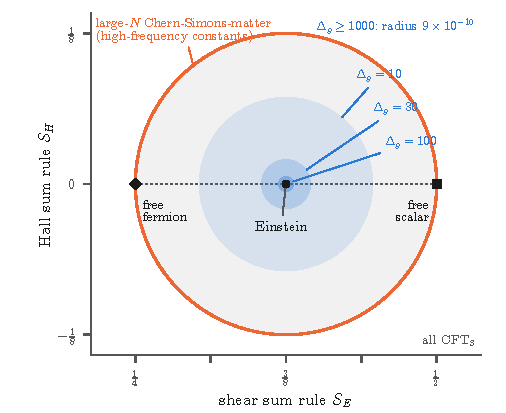
\includegraphics[width=\columnwidth]{fig/fig_disc}
\caption{\label{fig:disc}The thermal spectral weight of the stress tensor in the shear channel, $\mathcal S_E$, and in the
Hall channel, $\mathcal S_H$, both in units of the energy density. Every unitary CFT$_3$ satisfying the sum-rule conditions
lies in the grey disc. The free scalar and the free fermion sit at the ends of its horizontal diameter, large-$N$
Chern--Simons--matter theories on its rim, and Einstein gravity at its center. A higher-spin gap $\Delta_g$ confines a theory
with large $c_T$ to the blue disc of radius $\tau_*(\Delta_g)/32$, Eq.~\eqref{eq:angular}, shown for three gaps; at
$\Delta_g\ge1000$ the radius is $9\times10^{-10}$, Eq.~\eqref{eq:cubic}.}
\end{figure}

\textit{Thermal spectral weight}---Consider a unitary CFT$_3$ at temperature $T$, with energy density $\varepsilon$, and the
two shear components $T_1=(T_{xx}-T_{yy})/2$ and $T_2=T_{xy}$ at zero spatial momentum. Rotation invariance fixes their
retarded correlator to $G^R=\begin{pmatrix}g&-h\\h&g\end{pmatrix}$: $g$ describes ordinary shear response, and $h$, which is odd
under parity, the Hall response. At low frequency $g$ gives the viscosity $\eta$ and $h$ the Hall viscosity
$\eta_H$~\cite{Jensen:2011xb}. Subtracting the vacuum, we define the shear and Hall spectral weights
\begin{equation}
\mathcal S_E=\frac1{\pi\varepsilon}\!\int_{-\infty}^{\infty}\!\!d\omega\,\frac{\delta\rho(\omega)}{\omega},\quad
\mathcal S_H=\frac1{\pi\varepsilon}\!\int_{-\infty}^{\infty}\!\!d\omega\,\eta_H(\omega),
\label{eq:SEdef}
\end{equation}
where $\delta\rho={\rm Im}\,\delta g$ and $\eta_H(\omega)=-{\rm Im}\,\delta h(\omega)/\omega$ is the frequency-dependent Hall
viscosity. The three-point function $\langle TTT\rangle$ of a CFT$_3$ is fixed by $c_T$ and two
numbers~\cite{HofmanMaldacena,Buchel,CDPrakash}: $t_4$, and a parity-odd coefficient $\alpha_T$ that exists only in three
dimensions~\cite{GPY}. Both vanish for Einstein gravity, and we write $\tau=(t_4^2+\alpha_T^2)^{1/2}$.

Both integrals are fixed by the operator product expansion (OPE) at high frequency and by hydrodynamics at zero frequency. For
the shear channel, Chowdhury, David, and Prakash showed~\cite{Chowdhury:2016hjy} that
$\mathcal S_E=3/8+t_4/32$. For the Hall channel we find
\begin{equation}
|\mathcal S_H|=\frac{|\alpha_T|}{32}.
\label{eq:SH}
\end{equation}
The high-frequency tail of $\delta h$ is the exchange of $T$ with the parity-odd structure of $\langle TTT\rangle$, which in
three dimensions is the parity-even structure rotated by a helicity phase on the hard legs~\cite{Jain:2021gwa}; the rotation
turns the diagonal $t_4$ coefficient into an antisymmetric $\alpha_T$ coefficient of the same magnitude. We sketch this
argument and check it twice. On the AdS$_4$ black brane with the parity-odd cubic coupling, Eq.~\eqref{eq:SH} holds to
$10^{-3}$, and in the exactly solvable large-$N$ Chern--Simons--fermion theory~\cite{Ghosh:2019sqf} the high-frequency
coefficient matches $\alpha_T/32$ to $10^{-5}$ at every coupling tested. We also confirm the coefficient $1/32$ of $t_4$, which had not
been checked independently: exact free-field calculations give $\mathcal S_E=1/2$ for a free scalar ($t_4=4$) and $1/4$ for a free
fermion ($t_4=-4$), and a numerical calculation on the AdS$_4$ black brane gives $0.37499996$ for Einstein gravity~\cite{SM}.

The sum rules assume that no scalar of dimension at most three in $T\times T$ has a thermal expectation value, as in
Ref.~\cite{Chowdhury:2016hjy}; such a scalar adds a separate term. They give the frequency-integrated response exactly, at any
$c_T$. Combined with the conformal-collider bound $t_4^2+\alpha_T^2\le16$~\cite{CDPrakash}, which holds in every unitary
CFT$_3$, they give
\begin{equation}
\big(\mathcal S_E-\tfrac38\big)^2+\mathcal S_H^2\le\tfrac1{64}.
\label{eq:disc}
\end{equation}
Free fields saturate it on the horizontal axis, and large-$N$ Chern--Simons--matter theories, with $t_4+i\alpha_T=-4e^{-i\pi\lambda}$,
trace its whole boundary (Fig.~\ref{fig:disc}). Its parity-even projection, $1/4\le\mathcal S_E\le1/2$, was noted in
Ref.~\cite{Chowdhury:2016hjy}.

\textit{The higher-spin gap}---We now take $c_T$ large and assume three things. (i)~\emph{A higher-spin gap}: every
single-trace operator of spin four or more in $T\times T$ has twist at least $\Delta_g$; single traces of spin zero and two may
be light. (ii)~\emph{Weak coupling below the gap}: as $c_T\to\infty$ at fixed $\Delta_g$, the OPE of the unit-normalized $T$ with
itself below the gap is that of a generalized free field up to corrections that vanish uniformly in spin. Large-$N$
factorization gives this at each fixed spin; the uniformity in spin is the assumption, and no bulk effective theory is
assumed. (iii)~\emph{Positivity} of the functionals below on every heavy state, that is, every state of twist at least
$\Delta_g$. All bounds hold at leading order in $1/c_T$. We measure the gap by $\Lambda=[(\Delta_g-2)(\Delta_g-1)]^{1/2}$.

Two bounds on $\tau$ follow. Without any positivity input, commutativity of an energy detector with its first moment in
retarded time, together with crossing, gives at every gap
\begin{equation}
\tau\le\tau_*(\Delta_g):=\frac{160}{9(\Delta_g-2)}\Big[1-\frac{49}{(2\Delta_g+9)^2}\Big]^{-1/2}.
\label{eq:angular}
\end{equation}
This also needs that the detector identities hold as operator identities, that a mixed detector commutator converges in the
light-cone limit~\cite{KKSDZ}, and that no scalar of dimension at most one appears in $T\times T$. With positivity, which we
certify at $\Delta_g=1000$, and with no light single trace in $T\times T$,
\begin{equation}
\tau\le2.89\times10^{-8}\qquad(\Delta_g\ge1000),
\label{eq:cubic}
\end{equation}
by certified arithmetic $2.8914\times10^{-8}$. In the bulk, $\tau=240|\hat g_3|$, where $\hat g_3=\alpha_3+i\tilde\alpha_3$
combines the parity-even and parity-odd $R^3$ couplings of Ref.~\cite{CHLPS}, so $|\hat g_3|\Lambda^4\le120$. A theory with a
larger gap also has a gap of 1000, so Eq.~\eqref{eq:cubic} covers it. For a family of simpler functionals we prove positivity
analytically at every gap above 1000; given one further technical input they give
$\tau\le280\,[\log\frac{\Delta_g+2}3]^{1/2}(\Delta_g-2)^{-2}$~\cite{SM}.

\textit{Thermal spectroscopy bounds the spectrum}---The sum rules turn these vacuum bounds into statements about thermal
response. Write $\delta_{\rm th}=[(\mathcal S_E-3/8)^2+\mathcal S_H^2]^{1/2}=\tau/32$. Equation~\eqref{eq:angular} gives
$(\Delta_g-2)[1-49/(2\Delta_g+9)^2]^{1/2}\le5/(9\delta_{\rm th})$, so
\begin{equation}
\Delta_g\le2.2401+\frac5{9\,\delta_{\rm th}}.
\label{eq:gapthm}
\end{equation}
A CFT$_3$ with large $c_T$ whose thermal spectral weight departs from the Einstein value by $\delta_{\rm th}$ must contain a
single trace of spin four or more in $T\times T$ with twist below this value. A departure of $10^{-3}$ requires one below twist
558. The inequality uses no black brane and no positivity assumption. It holds under (i), (ii), the inputs of
Eq.~\eqref{eq:angular} and the sum-rule conditions; with $\mathcal S_E$ alone in place of $\delta_{\rm th}$ it does not use
Eq.~\eqref{eq:SH}. The gap discs of Fig.~\ref{fig:disc} are this statement. At $\Delta_g\ge1000$, Eq.~\eqref{eq:cubic} gives
$\delta_{\rm th}\le9.04\times10^{-10}$, and the analytic all-gap bound sharpens the reverse reading to
$\Delta_g\lesssim(8.75\sqrt{\log\Delta_g}/\delta_{\rm th})^{1/2}$: a departure of $10^{-12}$ requires a higher-spin state below
twist $5.8\times10^{6}$, rather than $5.6\times10^{11}$.

\textit{Hall viscosity without an axion}---The sum rules constrain integrated response. The transport coefficients
themselves need the dual geometry. We compute the shear and Hall viscosity of the planar AdS$_4$ black brane for the action
$R+6$ (in units of the AdS radius) plus all independent local curvature couplings through eight derivatives:
$-(\alpha_3J+\tilde\alpha_3Q)/6+(\alpha_4I^2+\alpha_4'P^2+2\tilde\alpha_4IP)/4$, with $I=C\cdot C$, $P=C\cdot\tilde C$, $J=C^3$, and
$Q=C^2\tilde C$ built from the Weyl tensor $C$ and its dual. With $\mathcal V=(4\pi\eta/s-1)-i\,4\pi\eta_H/s$, we find at first order
in the couplings
\begin{equation}
\mathcal V=18\,\hat g_3+216\,(\alpha_4+i\tilde\alpha_4).
\label{eq:V}
\end{equation}
The real part reproduces the known shear result~\cite{Li:2019auk}. The imaginary part is new: the parity-odd cubic coupling
$Q$, which is not a total derivative, produces a Hall viscosity on a neutral, isotropic brane, $4\pi|\eta_H|/s=(3/40)|\alpha_T|$.
Earlier holographic Hall viscosities needed an axion or a magnetic field~\cite{Saremi:2011ab,Hoyos:2019pyz}, and whether a
neutral holographic fluid can have one had not been studied systematically~\cite{Hoyos:2019pyz}. Here the answer is fixed by a
vacuum CFT datum. The coefficients were computed twice, with independent codes, and the response matrix is antisymmetric, as
Onsager reciprocity requires for a Hall coefficient~\cite{SM}.

Equation~\eqref{eq:V} turns the bound on $\tau$ into a bound on transport. Since $18|\hat g_3|=(3/40)\tau$ exactly, the cubic
coupling moves shear and Hall viscosity together along a circle. Flat-space causality bounds the quartic couplings by
$G_4=\alpha_4+\alpha_4'$~\cite{CHLPS,SM}, which the quartic sum rule bounds if the quartic functional is also positive. At
$\Delta_g\ge1000$,
\begin{equation}
|\mathcal V|\le\tfrac3{40}\tau+216\,G_4+\dots\le2.17\times10^{-9},
\label{eq:Vbound}
\end{equation}
so $|\eta_H|/s\le1.73\times10^{-10}$; the quartic part, $2\times10^{-14}$, is the only conditional piece. The second-order
terms are exact, $\mathcal V=\hat g_3(18-255\,{\rm Re}\,\hat g_3)+\dots$, and add at most $(17/3840)\tau^2=4\times10^{-18}$.

Unlike Eq.~\eqref{eq:gapthm}, this statement needs the bulk effective theory on the black brane, and that is a genuine
extra input: a coupling $I\,J$ of five gravitons is invisible in the vacuum three- and four-point functions yet shifts
$4\pi\eta/s$ by $-1944$ per unit coefficient. We therefore state the assumption in explicit form. If every coupling with $2k$
derivatives obeys $|\gamma|\le C\Lambda^{2-2k}$ for $k\ge5$, in the basis of Ref.~\cite{SM}, then the complete ten-derivative basis
and the infinite algebraic and gradient towers we can treat contribute at most $19300\,C/\Lambda^8=2\times10^{-20}C$ at
$\Delta_g=1000$. Even couplings $10^{9}$ times their natural size would not compete with Eq.~\eqref{eq:Vbound}.

\textit{A corrected viscosity bound}---In the helicity combinations $\eta-i\eta_H$ and $\mathcal S_E-i\mathcal S_H$ the cubic
coupling enters the viscosity and the sum rules with opposite signs, so it cancels from
\begin{equation}
\mathcal Z=\mathcal V+\tfrac{12}5\big(\mathcal S_E-\tfrac38-i\,\mathcal S_H\big)=216\,(\alpha_4+i\tilde\alpha_4)+\dots,
\label{eq:Z}
\end{equation}
and causality constrains what remains. Its real part gives
\begin{equation}
4\pi\frac\eta s\ \ge\ 1-\frac{12}5\Big(\mathcal S_E-\frac38\Big),
\label{eq:KSS}
\end{equation}
up to $(17/3840)t_4^2$ and the higher-derivative remainder above. The viscosity can fall below $1/4\pi$, as in the examples of
Refs.~\cite{Brigante:2007nu,Brigante:2008gz}, but only by an amount that the shear spectral weight measures; the sign of what is
left is fixed by the causality condition $\alpha_4\ge0$, a flat-space input that we assume in AdS. With the Hall channel included the allowed region is a disc tangent to
the origin, $|\mathcal Z-108G_4|\le108G_4$. The relative sign of the two channels in Eq.~\eqref{eq:Z} is not a convention; we
determined it from the full frequency dependence of the Hall correlator on the brane~\cite{SM}.

\begin{figure}[tb]
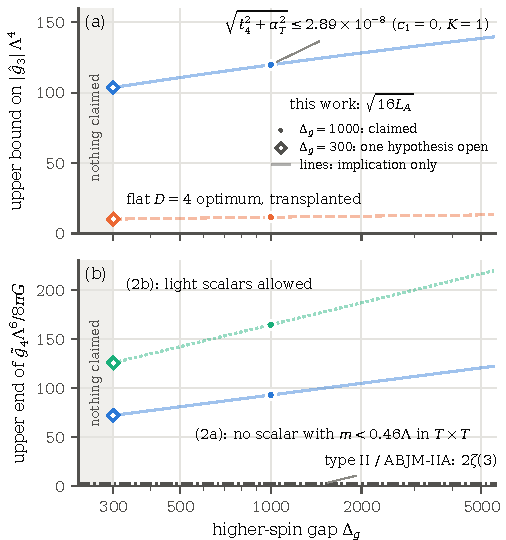
\includegraphics[width=\columnwidth]{fig/fig1_bounds}
\caption{\label{fig:bounds}Bounds as functions of the higher-spin gap. (a)~The bound on the deviation $\tau$ from Einstein
gravity, compared with the conformal-collider bound $\tau\le4$ and with the bound $\tau_*$ obtained without positivity, which sets
the radius $\tau/32$ of the gap discs in Fig.~\ref{fig:disc}. Dashed: the flat-space optimum of Ref.~\cite{CHLPS} transplanted to
AdS, shown for comparison; it is not an AdS bound. (b)~The upper bound on the $R^4$ coefficient with and without light scalars,
and the type~IIA string value $2\zeta(3)$ of ABJM theory. Filled circles: $\Delta_g=1000$. Faded lines: values that assume
positivity of the same functional at its own gap, established only at 1000. Purple: the analytic all-gap bounds (dashed: with a
further $k=3$ input).}
\end{figure}

\textit{How the bound on $\tau$ arises}---Light-transformed stress tensors~\cite{KSDlight} act as energy detectors at null
infinity, and two detectors commute when they are spacelike separated. Integrating the expectation value of their double
commutator against a weight gives a sum rule~\cite{KKSDZ,CLSD}, which converges in every unitary CFT~\cite{KKSDZ,CaronHuotInversion}.
We use it at finite $c_T$ and expand only its light part in $1/c_T$, as in Refs.~\cite{CHMRS,CLSD}. In the $T\times T$ OPE it
reads $\sum_{\rm heavy}(\text{OPE coefficient})^2\,\Omega(\text{state})=-\Omega(\text{light})$. The light side is the action
on the stress-tensor block alone, fixed by $c_T$ and $\tau$, because the double traces of $T$ sit at double zeros of the
functional. If $\Omega$ is positive on every heavy state, then $\Omega(\text{light})\le0$, and this inequality is
Eq.~\eqref{eq:cubic}. In flat space the condition reduces to the positivity used in Ref.~\cite{CHLPS}; in AdS, curvature moves
each heavy contribution away from its flat value, by amounts that are not small near the gap or at large impact parameter.

We rewrite the action of the functional on any heavy state exactly as a positive multiple of a finite ladder sum in each of
two helicity channels, and cover the infinite heavy spectrum at $\Delta_g=1000$ with certificates (Fig.~\ref{fig:coverage}).
Spins up to 1000 are certified one by one, high twist by an expansion about the leading-Regge value, and large spin near the twist
edge by three methods valid at large, intermediate, and small impact parameter. The difficulty is cancellation: the ladder
sum lies between about $10^{-5}$ and $10$ while its terms reach $10^{685}$. The large-spin certificates were rerun on separate
hardware with identical output, and a separate implementation of the rewriting agrees with direct evaluations at all 116
states computed earlier~\cite{SM}. Equation~\eqref{eq:angular} comes from a second sum rule in which an exact telescoping
identity makes every heavy contribution non-negative, so it needs no certificate.

\begin{figure}[tb]
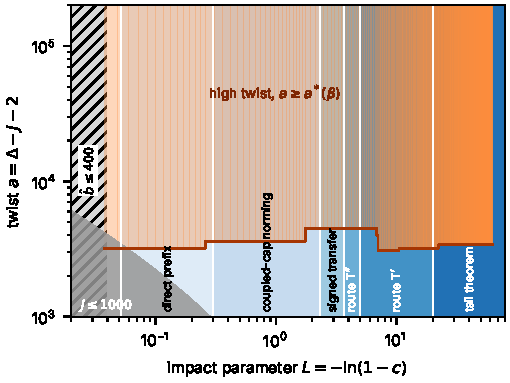
\includegraphics[width=\columnwidth]{fig/fig2_certificate}
\caption{\label{fig:coverage}Positivity of the functional on every heavy state at $\Delta_g=1000$: how certificates cover the
heavy spectrum, in the plane of twist and a logarithmic impact-parameter variable $L$ (large spin at fixed twist is large $L$).
Grey: spins up to 1000, certified one by one. Hatched: small impact parameter $\hat b$. Orange: twist above the high-twist
threshold $a^*$. Blue: the methods for large spin near the twist edge. Every region is certified~\cite{SM}.}
\end{figure}

\textit{What is not yet a theorem}---Three steps remain conditional. The quartic functional, which bounds $G_4$ in
Eq.~\eqref{eq:Vbound}, is positive on every state we have computed but is not certified. The CFT argument for
Eq.~\eqref{eq:SH} is a sketch, although it is checked in two independent theories. And the transport results need the bulk
effective theory on the brane. A CFT derivation of $\eta/s=1/4\pi$ up to powers of $1/\Delta_g$, which would remove that input, remains open; sum rules,
positivity and the KMS condition alone cannot provide it, and the Supplemental Material sets out what it requires~\cite{SM}.

In ABJM theory~\cite{ABJM} the gap is the string scale, and a gap of 1000 corresponds to a 't~Hooft coupling of about
$3\times10^9$. Supersymmetry sets $\tau=0$ there, and the string value of the $R^4$ coefficient is $2.6\%$ of our quartic bound
[Fig.~\ref{fig:bounds}(b)], a consistency check of the conditional part.

\textit{Conclusions}---In three dimensions the stress tensor's thermal spectral weight is a direct readout of the non-Einstein
part of its three-point function. Every CFT$_3$ lies in one disc, and a higher-spin gap confines a theory to a small disc about the
Einstein point, with a radius we compute. That makes thermal spectroscopy a probe of the higher-spin spectrum. In the dual fluid
the same coupling that rotates the three-point function produces a Hall viscosity, so shear and Hall response are pinned
together, to parts per billion at a gap of 1000. A combination of viscosity and spectral weight obeys a corrected version of the
viscosity bound, with its sign set by causality. The engine is a computer-assisted proof that a dispersive functional is positive
on the entire heavy spectrum of AdS at finite gap, together with a bound that needs no positivity. The method should carry over
to AdS$_5$/CFT$_4$, where the corresponding sum rules are known~\cite{Chowdhury:2016hjy} and $\mathcal N=4$ super-Yang--Mills
theory supplies exact checks.

\textit{Acknowledgments}---AI (Claude) assisted with the formulation and drafting of this manuscript. The authors take full
responsibility for the work presented, and have thoroughly reviewed all output.

\textit{Data availability}---The functional weights, the certificates with their inputs and outputs, and the
code that reproduces every constant are openly available~\cite{Zenodo}. The continuum weights given there as exact rationals define the functionals.

\bibliography{refs_verified,refs_v2}

\end{document}
